
%fitts metrics across groups, subjects and sessions
In this chapter the results processed from collected data will be presented. All data processing have been done in accordance to earlier introduced theory and implementations of methods described in \chapref{chap:Background} and \chapref{chap:Methods} respectively. Multiple comparison test of improvement across session of the two subject groups have been computed through a Friedman test, since the data proved to be non-Gaussian. When detecting an effect a Tukey-Kramer test was applied to correct for the problem of multiple comparison. Testing statistical differences between subject groups for each session was computed through a Mann-Witney U test. %All statistical analysis have been performed using MATLAB.


\section{Performance Results} \label{sec:R:fitts}
This section will present the results acquired from the Fitts' Law target reaching test described in \secref{sec:M:fittsLaw}. The test had five measures which each expresses a parameter of subjects' performance. Subjects were divided into two groups, one test group which received exact class confidence scores during user training, and a control group which only received label feedback. The plotted mean and standard deviations of each measure in the performance test for session can be seen in \figref{thereIsnoFigRefYet}.

\begin{figure}[H] 
	\subfigure[]
	{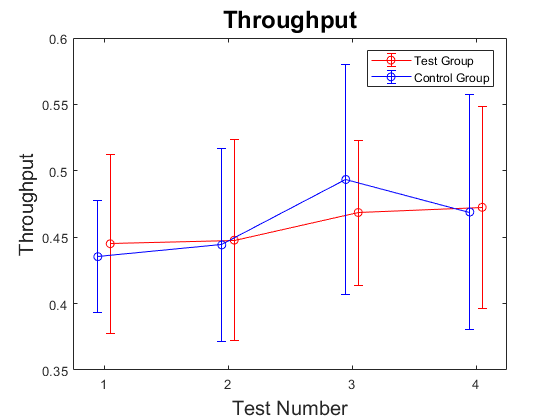
\includegraphics[width=.33\textwidth]{figures/xWesulds/Throughput}} 
	\hspace{-0.5cm}
	\subfigure[]
	{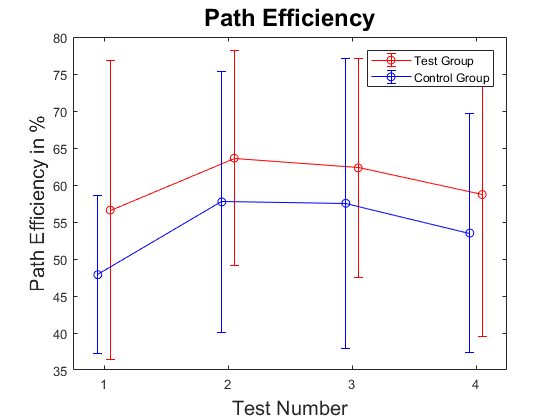
\includegraphics[width=.33\textwidth]{figures/xWesulds/PathEfficiency}} 
	\hspace{-0.5cm}
	\subfigure[]
	{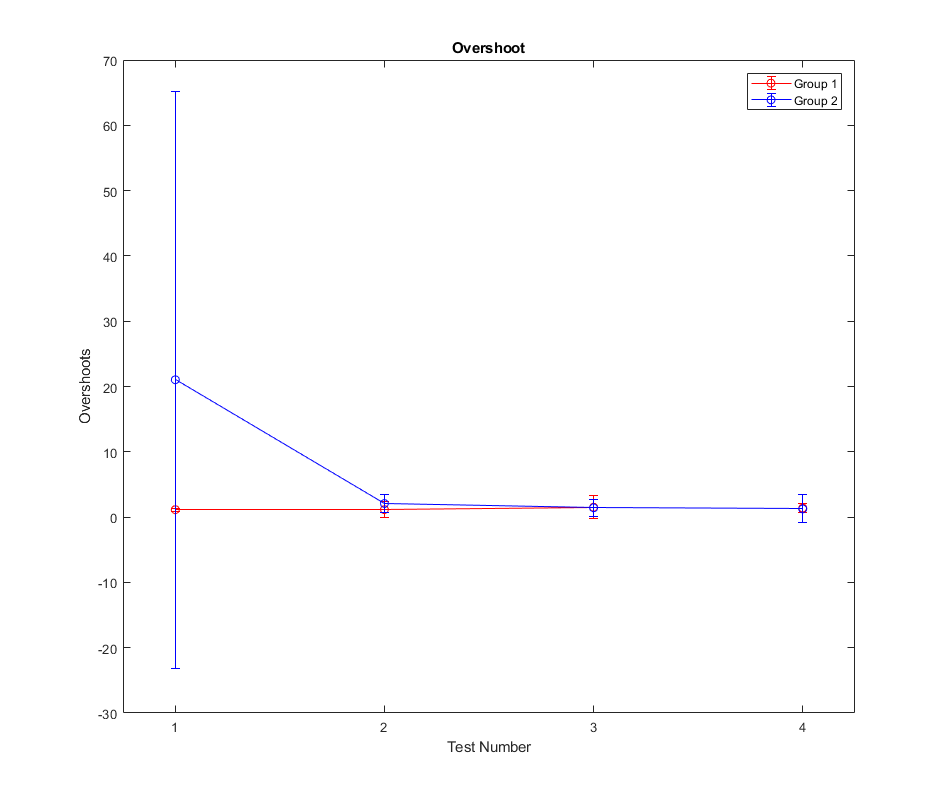
\includegraphics[width=.33\textwidth]{figures/xWesulds/Overshoot}}  
	\subfigure[]
	{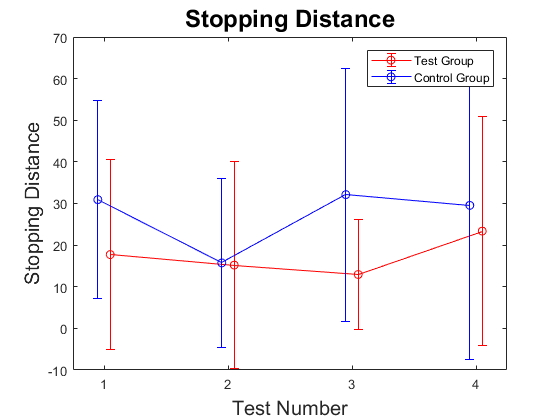
\includegraphics[width=.33\textwidth]{figures/xWesulds/StoppingDistance}} 
	\hspace{-0.5cm}
	\subfigure[]
	{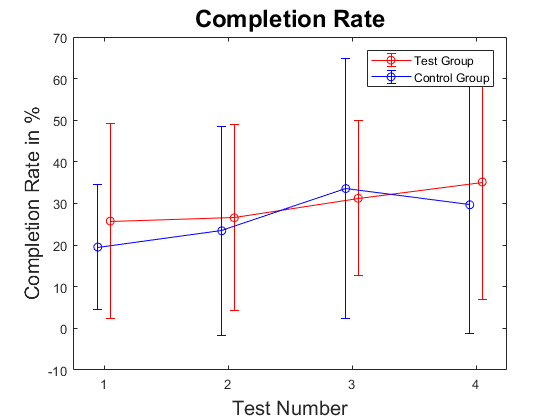
\includegraphics[width=.33\textwidth]{figures/xWesulds/CompletionRate}}  
	\hspace{-0.5cm}
	\caption{Figure illustrating the five performance measures; \textit{ a) Throughput, b) Path efficiency, c) Overshoot, d) Stopping distance, e) Completion rate}, used for quantifying user performance across all four tests.  Test number 1 is the acquired baseline used for assessing group homogeneity and the following numbers indicate performance test results after user training in each session. The red line indicates the progression of the test group and the blue of the control group.}
	\label{thereIsnoFigRefYet}
	
\end{figure}
	

The aim of using the Fitts' Law target reaching test was to apply a method to quantitatively evaluate the performance of subjects after user training in each session. The information drawn from the measures are described in \secref{sub:BG:fitts}. The baseline performance test showed no difference between the two group, showing the two groups to be homogeneous at initiation. The Fitts' Law test results did not show any significant improvement over the three sessions for any of the five test measures for both the test and control group ($p > 0.05$). Similarly, there was no significant difference between the two groups performance in any sessions ($p > 0.05$), meaning neither of them performed significantly better than the other group in any of the sessions.
%\subsection{Between test and control group}
%Here the results from the Fitts' Law targets reaching test between the two groups will be presented.

%throughput
%\begin{figure}[H] 
%	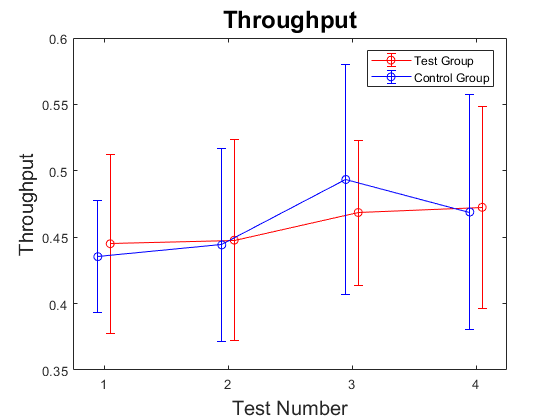
\includegraphics[width=0.4\textwidth]{figures/xWesulds/Throughput}
%	\caption{Throughput metric for the Fitts' Law test between the test and control group.}
%	\label{fig:TPresult}
%\end{figure}
%
%%Path Efficiency
%\begin{figure}[H] 
%	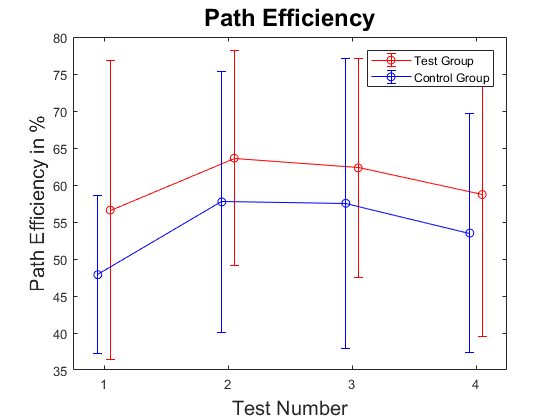
\includegraphics[width=0.4\textwidth]{figures/xWesulds/PathEfficiency}
%	\caption{Path efficiency metric for the Fitts' Law test between the test and control group.}
%	\label{fig:PEresult}
%\end{figure} 

% No significant difference were found between any groups performance of any of the performance metrics ($p > 0.05$).  %throughput or path efficiency. 
%Here the subjects throughput metric inform of the subjects balance of speed and accuracy, as described in \secref{sub:BG:fitts}. Subjects path efficiency measure how well subjects

%\begin{figure}[H] 
%	\centering
%	\subfigure[Throughput metric for the Fitts' Law test between the test and control group. There is no significant difference between the groups ($p > 0.05$).]
%	{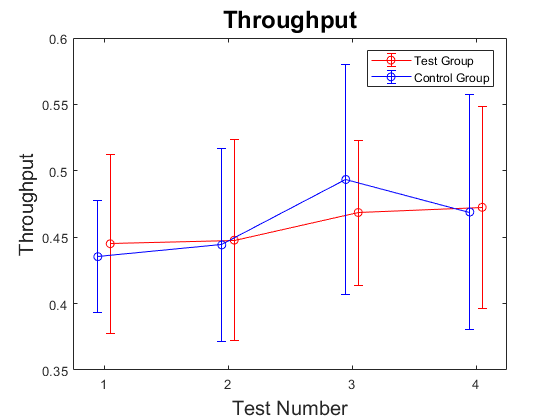
\includegraphics[width=.49\textwidth]{figures/xWesulds/Throughput}}
%	\subfigure[Path efficiency metric for the Fitts' Law test between the test and control group. There is no significant difference between the groups ($p > 0.05$).]
%	{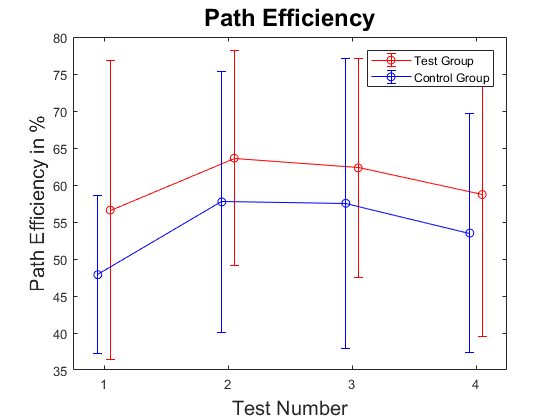
\includegraphics[width=.49\textwidth]{figures/xWesulds/PathEfficiency}}  
%	\caption{Presentation of the result metrics throughput and path efficiency.}
%	\label{fig:resultsTP_PE}
%\end{figure}

%overshoot
%\begin{figure}[H] 
%	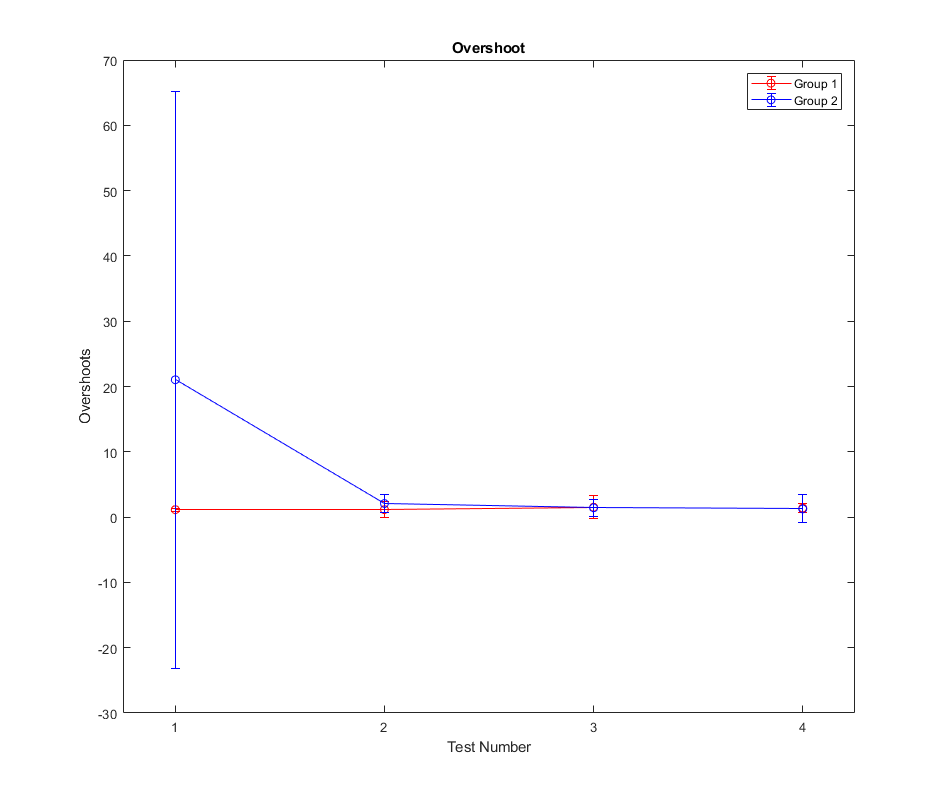
\includegraphics[width=0.4\textwidth]{figures/xWesulds/Overshoot}
%	\caption{Overshoot metric for the Fitts' Law test between the test and control group.}
%	\label{fig:OSresult}
%\end{figure} 
%
%%stopping distance
%\begin{figure}[H] 
%	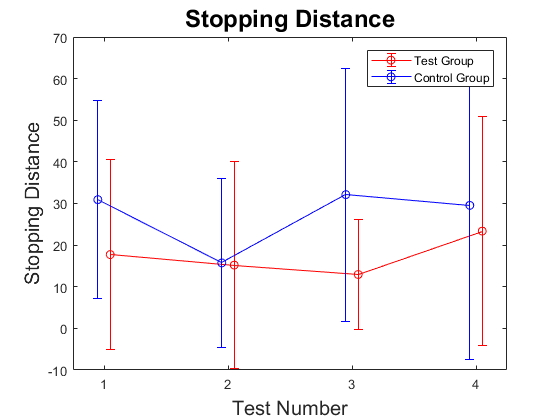
\includegraphics[width=0.4\textwidth]{figures/xWesulds/StoppingDistance}
%	\caption{Stopping distance metric for the Fitts' Law test between the test and control group.}
%	\label{fig:SDresult}
%\end{figure} 

%\begin{figure}[H] 
%	\centering
%	\subfigure[Overshoot metric for the Fitts' Law test between the test and control group. There is no significant difference between the groups ($p > 0.05$).]
%	{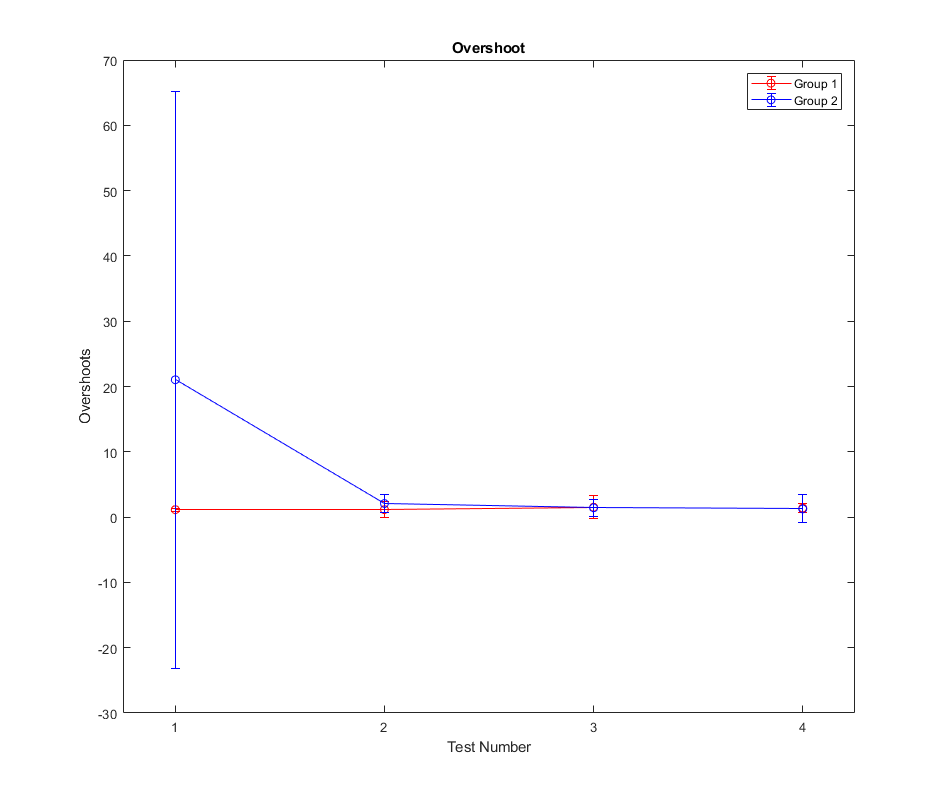
\includegraphics[width=.49\textwidth]{figures/xWesulds/Overshoot}}
%	\subfigure[Stopping distance metric for the Fitts' Law test between the test and control group. There is no significant difference between the groups ($p > 0.05$).]
%	{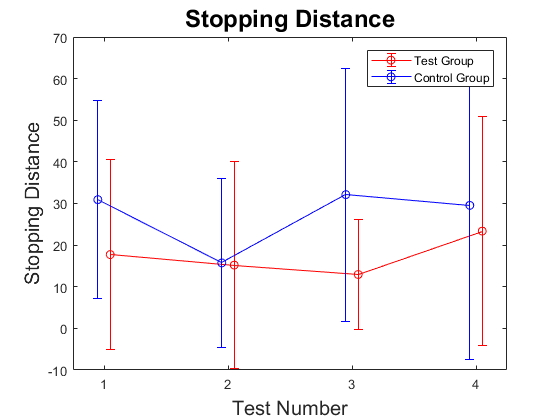
\includegraphics[width=.49\textwidth]{figures/xWesulds/StoppingDistance}}  
%	\caption{Presentation of the result metrics overshoot and stopping distance.}
%	\label{fig:resultsOS_SD}
%\end{figure}
%
%%completion rate
%\begin{figure}[H] 
%	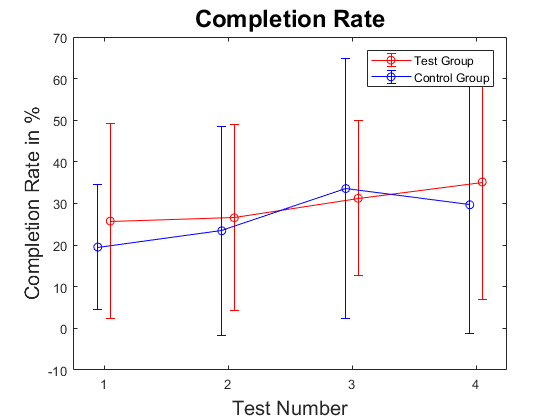
\includegraphics[width=0.49\textwidth]{figures/xWesulds/CompletionRate}
%	\caption{Completion rate metric for the Fitts' Law test between the test and control group. There is no significant difference between the groups ($p > 0.05$).}
%	\label{fig:CRresult}
%\end{figure} 

%\subsection{Across sessions}

%No significant difference in performance was found between the four tests with $p > 0.05$ for both the overall Friedmans test and the Tukey-Kramer correction to test difference between each session. This was the case for both the test and control group, which means there was no significant development of performance between either of the sessions for any group.

